\chapter{面向碳纳米管阵列研究的知识建模与检索增强方法}
\enchapter{Knowledge Modeling and Retrieval Augmentation Methods for Carbon Nanotube Array Research}
\label{chap:knowledge_method}

\section{引言}
\ensection{Introduction}

碳纳米管阵列研究涉及工艺参数调控、形貌特征表征、生长机理分析与材料性能评估等多个环节，不同环节之间存在明显的条件依赖关系与因果传递关系。随着大语言模型和检索增强生成技术的发展，利用外部知识支撑科研分析成为可能。然而，在碳纳米管阵列这类专业性强、机理链条复杂、实验条件敏感的研究场景中，通用文本块式检索增强方法仍存在明显局限：其通常以固定长度文本片段作为基本检索单元，难以显式保留“工艺参数—生长机理—形貌特征—材料性能”之间的局部科研事实结构，也难以满足面向条件约束和关系约束的精确检索需求。由此，在进行形貌解释、规律归纳或结果分析时，模型容易检索到语义相关但结构割裂的证据片段，从而影响分析结果的准确性、可追溯性与可解释性。

针对上述问题，本章提出一种面向碳纳米管阵列研究的知识建模与检索增强方法。本章不追求构建复杂的图学习模型，而是以最小语义事实单元为基础，通过轻量级领域关系结构和任务约束检索机制，实现面向科研分析任务的链式证据组织与调用。具体而言，本章的方法主线包括以下三个环节：
\begin{enumerate}
    \item \textbf{多源知识规范化与层次化切分。}面向学术文献、实验记录、工艺参数表、结构化实验数据及图像分析结果，构建多源知识规范化处理流程，并设计面向科研事实的层次化切分方法，将异构原始知识转化为统一、可关联的候选知识片段。
    \item \textbf{科研事实表示与领域关系建模。}提出最小语义事实单元表示方法，并建立核心对象、关系类型与约束规则组成的轻量级领域关系结构，实现对“工艺参数—生长机理—形貌特征—材料性能”等关键科研关系的结构化表达。
    \item \textbf{面向科研任务的检索增强算法。}在上述知识表示基础上，设计面向科研任务的检索增强方法，通过混合召回、关系约束扩展与路径重排序，生成支持科研分析与结果解释的链式证据集合。
\end{enumerate}

在此基础上，第 3.4 节进一步给出面向上述方法的评测设计，用于验证知识单元建模与链式证据检索的有效性。需要说明的是，本章输出的并不是最终科研结论，而是为后续结果解释与规律归纳提供证据基础。图~\ref{fig:3_1} 给出了本章方法的整体框架，其主要包括知识规范化与事实单元构建、关系约束检索与证据生成，以及对应的评测安排三个层次。

\begin{figure}[htbp]
    \centering
    \includegraphics[width=0.95\textwidth]{figures/3.1.png}
    \caption{面向碳纳米管阵列研究的知识建模与检索增强框架}
    \label{fig:3_1}
\end{figure}

\section{面向碳纳米管阵列研究的知识单元建模方法}
\ensection{Knowledge Unit Modeling Method for Carbon Nanotube Array Research}

为支撑后续关系约束检索与证据组织任务，需要将来源分散、形式异构且语义粒度不一致的原始知识转化为统一、可关联的结构化表示。针对碳纳米管阵列研究中学术文献、实验记录、工艺参数表、结构化数据库及图像表征结果并存的特点，本文围绕多源知识规范化、面向科研事实的层次化切分、最小语义事实单元构建以及核心对象—关系规则建模四个方面开展知识表示研究。规范化处理的目标不是保留所有原始格式细节，而是将不同来源知识统一映射为后续切分、抽取与索引所需的中间表示。

\subsection{多源知识规范化处理}
\ensubsection{Normalized Processing of Multi-source Knowledge}

碳纳米管阵列研究中的原始知识来源主要包括学术文献、实验记录与工艺参数表、结构化实验数据库以及图像表征结果。由于不同来源数据在文件格式、字段组织方式和语义表达粒度上存在显著差异，若直接作为后续知识建模的输入，容易导致同类信息表示不一致、样品标识无法对齐以及上下文语义缺失等问题。为此，本文设计一套面向多源异构知识的规范化处理流程，将不同来源知识统一转换为结构一致、字段清晰的标准化中间表示。

设原始多源知识集合为
\begin{equation}
    D=\{d_k\}_{k=1}^{N}
\end{equation}
其中，$d_k$ 表示第 $k$ 个原始知识对象。本文通过规范化映射函数 $F_{\mathrm{norm}}(\cdot)$ 将原始知识对象统一转换为规范化知识对象：
\begin{equation}
    \tilde{d}_k=F_{\mathrm{norm}}(d_k)
\end{equation}
其中，$\tilde{d}_k$ 表示经过格式清洗、字段对齐和标识统一后的规范化对象。为明确规范化阶段的统一输出形式，本文进一步将任一规范化对象表示为
\begin{equation}
    \tilde{d}_k=(x_k,\, m_k,\, f_k)
\end{equation}
其中，$x_k$ 表示可供后续切分的规范化文本主体；$m_k$ 表示来源标识、样品编号、来源类型、时间或年份等元数据；$f_k$ 表示已经完成字段对齐的结构化内容，如工艺参数、形貌指标、性能指标和机理术语等。无论原始来源是文献段落、实验记录、参数表还是图像分析结果，规范化阶段均输出上述统一结构，从而为后续切分、事实单元构建与索引组织提供一致输入。

针对不同类型的数据源，本文采用差异化但口径统一的规范化处理策略。学术文献以段落或句群为基本处理单元，重点完成版式去噪、术语归一化和来源信息保留；实验记录与工艺参数表以样品编号或批次编号为主键，重点完成参数项、单位和值的统一映射；结构化实验数据库以记录行为规范化对象，重点完成字段对齐、缺失值处理和主键关联；图像表征结果则直接以量化后的形貌指标作为结构化输入。四类数据源的具体处理口径如表~\ref{tab:3_1_norm_sources} 所示。

\begin{table}[htbp]
    \centering
    \caption{多源知识规范化对象及处理口径}
    \label{tab:3_1_norm_sources}
    \renewcommand{\arraystretch}{1.3}
    \setlength{\tabcolsep}{5pt}
    \begin{tabular}{p{2.4cm} p{2.6cm} p{4.5cm} p{4.0cm}}
        \toprule
        \textbf{数据源类型} & \textbf{基本处理对象} & \textbf{规范化动作} & \textbf{统一输出重点} \\
        \midrule
        学术文献 & 段落或句群 & 版式去噪、术语归一化、章节位置保留、参考信息抽取 & 文本主体 $x_k$ 及文献来源元数据 $m_k$ \\
        \midrule
        实验记录与工艺参数表 & 样品编号或批次编号对应记录 & 参数项对齐、单位统一、数值映射、记录位置保留 & 结构化参数字段 $f_k$ 及样品级元数据 $m_k$ \\
        \midrule
        结构化实验数据库 & 单条记录行 & 字段对齐、缺失值处理、主键关联、跨表整合 & 围绕样品实体组织的结构化字段 $f_k$ \\
        \midrule
        图像表征结果 & 已量化的形貌指标记录 & 样品绑定、来源绑定、表征条件绑定 & 取向度、平均曲率、覆盖密度、直径分布等字段写入 $f_k$ \\
        \bottomrule
    \end{tabular}
\end{table}

多源异构知识规范化处理流程如图~\ref{fig:3_2_norm_flow} 所示。通过上述处理，原本分散且异构的多源知识被转换为统一的规范化对象集合，为后续层次化切分、跨源样品对齐和关系抽取提供了一致输入。

\begin{figure}[H]
    \centering
    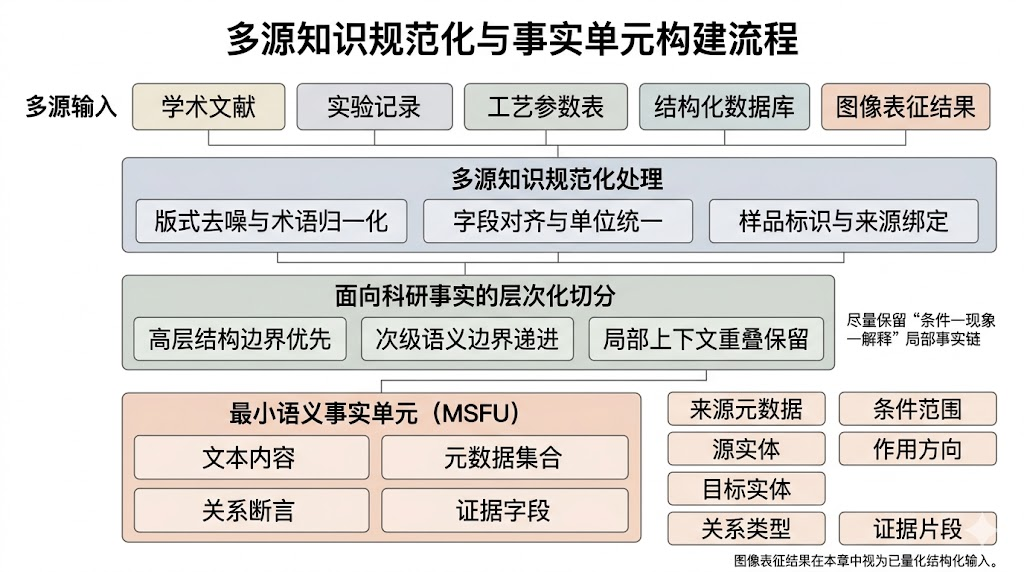
\includegraphics[width=0.92\textwidth]{figures/3.2.jpg}
    \caption{多源知识规范化与事实单元构建流程示意图}
    \label{fig:3_2_norm_flow}
\end{figure}

\subsection{面向科研事实的层次化切分方法}
\ensubsection{Hierarchical Segmentation Method Based on Scientific Facts}

在完成多源知识规范化处理后，需要将长文本转换为适合信息抽取的候选片段。对于碳纳米管阵列研究语料而言，单个文本段落中往往同时包含工艺条件、实验现象及机理解释等多类信息。若采用固定长度或滑动窗口的普通切分方式，容易破坏“条件—现象—解释”这一局部科研事实链条。为此，本文设计了一种面向科研事实的层次化切分方法，其目标是在满足模型处理长度约束的同时，尽可能保留局部事实表达的完整性。

设规范化后的知识对象 $\tilde{d}_k$ 对应文本内容为 $x_k$，本文定义分段映射函数 $F_{\mathrm{seg}}(\cdot)$，将其转换为候选片段集合：
\begin{equation}
    C_k=F_{\mathrm{seg}}(x_k)=\{c_{k,j}\}_{j=1}^{M_k}
\end{equation}
其中，$c_{k,j}$ 表示从第 $k$ 个知识对象中切分得到的第 $j$ 个候选片段，$M_k$ 表示该对象切分后的片段总数。与仅以长度为依据的滑动窗口切分不同，本文优先依据科研事实边界进行分段，以尽量保留“条件—现象—解释”的局部表达完整性。

该方法遵循“高层结构边界优先、次级语义边界递进、局部上下文重叠保留”的原则。首先，优先依据段落换行、小节标题、实验步骤和参数列表等高优先级结构边界进行初始划分，以避免截断完整论述单元。其次，当初步得到的片段长度仍超过预设阈值时，再沿句号、分号及并列参数项边界进行递归细分，使片段在满足长度约束的同时保持局部语义连续性。最后，为减弱硬性切分对指代关系和上下文依赖的影响，在相邻片段之间保留局部重叠窗口。设单个片段允许的最大长度为 $L_{\max}$，相邻片段之间保留的重叠长度为 $r$，则有：
\begin{equation}
    L(c_{k,j})\leq L_{\max}
\end{equation}
\begin{equation}
    c'_{k,j}= \mathrm{tail}_{r}(c_{k,j-1}) \oplus c_{k,j}
\end{equation}
其中，$\mathrm{tail}_{r}(\cdot)$ 表示取前一片段末尾长度为 $r$ 的文本，$\oplus$ 表示文本拼接操作。参数 $L_{\max}$ 由后续编码模型的输入长度约束与单条科研事实的完整表达需求共同确定，用于避免片段过长而影响抽取稳定性；参数 $r$ 用于保留相邻片段之间的局部上下文，通常取能够覆盖条件短语、指代成分或句间承接信息的最小窗口。为避免后文记号切换造成歧义，下文中凡指经过重叠增强后的最终片段，均统一记作 $c_{k,j}$。

与传统固定长度切分相比，该方法生成的片段不再是彼此割裂的文本块，而是保留局部科研逻辑结构的候选表达单元，并作为后续最小语义事实单元构建与关系抽取的稳定输入。

\subsection{最小语义事实单元表示}
\ensubsection{Representation of Minimum Semantic Fact Unit}

在获得保留局部逻辑的候选片段后，仍需进一步将非结构化文本转化为可检索、可关联的科研事实表示。传统文本片段主要支持基于关键词或向量相似度的检索方式，难以显式表达知识内部的对象关系、作用方向和条件约束。为此，本文提出最小语义事实单元（Minimum Semantic Fact Unit, MSFU）表示方法，用于将候选片段组织为面向科研分析任务的结构化知识单元。本文仅对最小语义事实单元的文本内容及扩展语义字段进行向量化表示，用于支持语义召回；其关系断言及约束信息保留为符号化表示，用于后续关系约束扩展与证据链组织。

对于由第 $k$ 个知识对象切分得到的第 $j$ 个候选片段 $c_{k,j}$，其对应的最小语义事实单元定义为：
\begin{equation}
    u_{k,j}=(c_{k,j},\, m_{k,j},\, a_{k,j},\, e_{k,j})
\end{equation}
其中，$c_{k,j}$ 为原始候选片段文本；$m_{k,j}$ 为元数据集合，用于记录来源、主题类别、任务标签等信息；$a_{k,j}$ 为关系断言结构，用于表达片段中包含的核心对象关系；$e_{k,j}$ 为证据集合，用于支持后续证据追溯与结果验证。

其中，关系断言结构 $a_{k,j}$ 进一步表示为：
\begin{equation}
    a_{k,j}=(e^{src}_{k,j},\, r^{type}_{k,j},\, e^{tgt}_{k,j},\, cond_{k,j},\, dir_{k,j})
\end{equation}
其中，$e^{src}_{k,j}$ 表示源实体，$e^{tgt}_{k,j}$ 表示目标实体，$r^{type}_{k,j}$ 表示关系类型，$cond_{k,j}$ 表示关系成立的条件范围，$dir_{k,j}$ 表示作用方向或变化趋势。通过上述定义，原始文本中的“在何种条件下，哪个对象通过何种关系作用于哪个对象，并表现出何种变化”得到了统一表达。需要进一步说明的是，$c_{k,j}\rightarrow u_{k,j}$ 的构建并非人工直接给定，而是通过“领域词表与规则模板初筛 + 轻量实体识别与关系识别 + 必要时大语言模型辅助补全 + 人工抽样校验”完成。具体而言，系统首先利用领域术语词表、条件触发词和方向模式识别候选实体与条件短语，再通过轻量级实体/关系抽取模块生成源实体、目标实体和关系类型候选；对于存在省略、跨句指代或复合比较关系的片段，则使用大语言模型辅助补全条件范围与变化方向；最后通过人工抽样校验修正规则与术语表，以保证事实单元构建具有较好的工程可复现性。

例如，对于片段文本 $c_{k,j}$：
\begin{quote}
提高生长温度后，碳纳米管阵列取向度提升，可能与催化剂活性增强有关。
\end{quote}
可将其表示为
\begin{equation}
    u_{k,j}=(c_{k,j},\, m_{k,j},\, a_{k,j},\, e_{k,j})
\end{equation}
其中，关系断言可写为
\begin{equation}
    a_{k,j}=(\text{生长温度},\, \text{促进},\, \text{取向度},\, \text{温度升高},\, \text{上升})
\end{equation}
扩展语义字段中记录 $\mathrm{mechanism\_terms}=\{\text{催化剂活性增强}\}$，证据字段中记录
\begin{equation}
    e_{k,j}=(\text{evidence\_span}=c_{k,j},\, \text{keywords}=\{\text{生长温度},\, \text{取向度},\, \text{催化剂活性}\})
\end{equation}
若该片段来自学术文献，则其元数据 $m_{k,j}$ 中还可保留 $\mathrm{doc\_id}$、$\mathrm{source\_type}$、$\mathrm{title}$ 和 $\mathrm{theme}$ 等字段。通过这种写法，同一事实片段被完整映射为“文本主体—关系断言—证据字段”的统一结构，而不再停留在自然语言解释层面。

该表示方式一方面保留了原始文本与元数据，能够支持来源追溯与语境恢复；另一方面将对象关系及约束条件显式化，使后续检索能够在“实体—关系—条件”层面进行筛选，而不再仅依赖文本相似度。关系断言中的实体可映射为后续关系结构中的节点，关系类型、条件范围、作用方向以及证据强度等信息则作为边属性进入后续路径扩展与路径筛选。

需要说明的是，并非所有候选片段都能够抽取出完整的关系断言。对于无法识别出明确源实体、目标实体或关系类型的片段，本文仅保留其文本与元数据索引，不将其纳入关系结构索引；而对于能够形成完整关系表达的片段，则构造成最小语义事实单元并进入后续关系检索流程。表~\ref{tab:3_1_unit_schema} 给出了最小语义事实单元的主要字段设计及其作用说明。

\begin{table}[htbp]
    \centering
    \caption{最小语义事实单元字段设计及其作用说明}
    \label{tab:3_1_unit_schema}
    \renewcommand{\arraystretch}{1.3}
    \setlength{\tabcolsep}{6pt}
    \begin{tabular}{p{2.5cm} p{5.5cm} p{5.0cm}}
        \toprule
        \textbf{字段类别} & \textbf{字段组成} & \textbf{主要作用} \\
        \midrule
        元数据字段
        & 文档标识（doc\_id）、标题（title）、样品编号（sample\_id）、批次编号（batch\_id）、来源类型（source\_type）、实验体系（experiment\_system）、主题类别（theme）、任务标签（task\_tag）、年份（year）
        & 支持来源过滤、样品级对齐、实验体系约束与任务定向检索 \\
        \midrule
        语义字段
        & 源实体（source\_entity）、目标实体（target\_entity）、关系类型（relation\_type）、作用方向（effect\_direction）、条件范围（condition\_scope）
        & 支撑对象关系检索、路径筛选与结构化分析 \\
        \midrule
        扩展语义字段
        & 机制术语（mechanism\_terms）、性能术语（performance\_terms）
        & 增强机理解释与性能分析场景下的语义识别能力 \\
        \midrule
        证据字段
        & 证据片段（evidence\_span）、关键词（keywords）、置信度（confidence）、核心性标记（is\_core）
        & 支撑结果验证、证据追溯与证据强度评估 \\
        \bottomrule
    \end{tabular}
\end{table}

\subsection{核心对象、关系类型与约束规则建模}
\ensubsection{Modeling of Core Objects, Relation Types, and Constraint Rules}

在确立最小语义事实单元表示后，还需要从全局层面对知识单元进行统一组织，以避免海量事实单元在检索与推理过程中出现无序聚合。结合碳纳米管阵列材料生长研究的领域特点，本文进一步定义核心对象类别、关系类型以及约束规则，构成面向碳纳米管阵列研究的轻量级领域关系结构。

首先，本文将领域中的关键对象抽象为四类核心对象：工艺实体、形貌实体、性能实体和机理实体。工艺实体主要描述实验输入条件与调控参数，如生长温度、退火时间、催化剂厚度、缓冲层厚度和气体流量等；形貌实体用于表征碳纳米管阵列的结构特征，包括取向度、平均曲率、覆盖密度和直径分布；性能实体用于描述材料在应用端表现出的宏观指标，如导电性、电阻率、拉伸强度和弹性模量；机理实体则用于表示影响生长与演化过程的微观机制，如催化剂失活、扩散受限、边界层效应、颗粒团聚和奥斯特瓦尔德熟化等。表~\ref{tab:3_2_entities} 给出了各类核心对象的典型示例。

\begin{table}[htbp]
    \centering
    \caption{核心对象类别及示例说明}
    \label{tab:3_2_entities}
    \renewcommand{\arraystretch}{1.3}
    \setlength{\tabcolsep}{6pt}
    \begin{tabular}{p{2.5cm} p{5.5cm} p{5.0cm}}
        \toprule
        \textbf{对象类别} & \textbf{典型示例} & \textbf{说明} \\
        \midrule
        工艺实体 & 生长温度、退火时间、催化剂厚度、缓冲层厚度、气体流量、催化剂状态 & 描述实验输入条件与工艺调控参数 \\
        \midrule
        形貌实体 & 取向度、平均曲率、覆盖密度、直径分布 & 描述碳纳米管阵列的结构特征 \\
        \midrule
        性能实体 & 导电性、电阻率、拉伸强度、弹性模量 & 描述材料在应用端的宏观性能指标 \\
        \midrule
        机理实体 & 催化剂失活、扩散受限、边界层效应、颗粒团聚、奥斯特瓦尔德熟化、应力诱导弯曲 & 描述影响生长演化的微观物理化学机制 \\
        \bottomrule
    \end{tabular}
\end{table}

在此基础上，本文进一步定义五类主要关系类型，用于刻画不同对象类别之间的语义关联。第一类为工艺—形貌关系，用于描述工艺参数变化对阵列形貌特征的影响；第二类为形貌—性能关系，用于表达形貌结构对材料性能的作用；第三类为工艺—性能关系，用于表示工艺条件与宏观性能之间的直接关联；第四类为工艺—机理关系，用于刻画工艺调控对微观机制的触发或抑制作用；第五类为机理—形貌关系，用于表示微观机制如何进一步影响最终形貌。上述关系类型共同构成了碳纳米管阵列研究中的基本知识传递路径。

为保证关系调用和多跳扩展的有效性，本文进一步引入四类约束规则。其一为链路约束，用于限定允许的关系连接方式，避免出现不符合领域逻辑的跨类跳转；其二为方向约束，用于约束关系的作用方向，防止产生与物理过程不一致的逆向推断；其三为条件约束，用于要求关系在满足特定条件范围时才被判定为有效，如温度区间、催化剂状态或气体比例等；其四为任务约束，用于根据具体任务类型控制可调用的关系类型和路径范围，例如形貌解释任务与性能分析任务所关注的关系链条并不完全相同。表~\ref{tab:3_3_relations_rules} 对各类关系与约束规则进行了说明。

\begin{table}[htbp]
    \centering
    \caption{关系类型与约束规则说明}
    \label{tab:3_3_relations_rules}
    \renewcommand{\arraystretch}{1.3}
    \setlength{\tabcolsep}{6pt}
    \begin{tabular}{p{3.0cm} p{5.5cm} p{4.5cm}}
        \toprule
        \textbf{类别} & \textbf{名称} & \textbf{含义与约束说明} \\
        \midrule
        关系类型
        & 五类对象间主关系
        & 描述工艺、形貌、性能、机理间的主要语义关联与知识传递路径 \\
        \midrule
        约束规则
        & 链路约束、方向约束、条件约束、任务约束
        & 限定关系扩展方式、作用方向、成立条件及任务适用范围，支撑后续路径扩展与路径筛选 \\
        \bottomrule
    \end{tabular}
\end{table}

通过上述建模，本文为后续关系约束检索提供了统一的模式层表示。核心对象定义节点类型，关系类型规定语义连接方式，链路约束与任务约束共同决定第 3.3 节任务转移矩阵 $A_t$ 中可接受的关系转移；条件约束和方向约束则分别转化为 $S_{\mathrm{cond}}(q,e)\geq \tau_c$ 与 $S_{\mathrm{dir}}(q,e)\geq \tau_d$ 的筛选条件。

\section{面向碳纳米管阵列研究的检索增强方法}
\ensection{Retrieval-Augmented Method for Carbon Nanotube Array Research}

在完成多源知识规范化、最小语义事实单元表示以及核心对象、关系类型与约束规则建模后，知识库已具备结构化表示基础。但仅有知识表示仍不足以直接支撑复杂科研问题中的精准分析。为此，本文进一步提出面向碳纳米管阵列研究的检索增强方法。本节以约束链式证据检索算法 TCCER 为统一主线，说明如何在任务约束下从最小语义事实单元中召回候选知识、沿关系约束扩展为证据路径，并最终组织为链式证据集合。这里的关系图仅用于任务约束、条件筛选和证据组织，而不是用于复杂图表示学习。

\subsection{研究任务定义与检索需求分析}
\ensubsection{Research Task Definition and Retrieval Requirement Analysis}

结合碳纳米管阵列研究中的典型场景，本文将检索增强所服务的核心任务归纳为以下三类：

\begin{enumerate}
    \item \textbf{工艺分析任务。}
    该类任务主要关注特定工艺参数或工艺组合对碳纳米管阵列形貌和性能的影响规律，例如温度变化对取向度的影响、催化剂厚度变化对直径分布的作用，以及不同气流比条件下覆盖密度的变化等。对于此类任务，检索结果应能够准确关联目标工艺变量与形貌特征或性能指标，并尽可能保留作用方向、条件范围和证据来源等关键信息，以支持参数比较、规律归纳和工艺优化分析。

    \item \textbf{形貌解释任务。}
    该类任务主要针对实验观测到的形貌现象，分析其潜在成因及相关机理，例如覆盖密度下降可能对应的机理变化、平均曲率增大是否与碳供给不均有关，以及取向度降低是否与催化剂失活或扩散受限相关等。与工艺分析任务相比，形貌解释任务更强调工艺参数、生长机理和形貌特征之间的链式支撑，因此检索结果不仅应具有语义相关性，还应具有较好的链路完整性和结构一致性。

    \item \textbf{预测解释任务。}
    该类任务面向第四章中的形貌预测结果，关注如何利用领域知识对模型输出进行辅助说明与合理性分析。例如，当模型预测某组工艺参数下取向度下降、平均曲率增大或直径分布增宽时，需要进一步说明该预测趋势是否能够从已有实验规律、生长机理或文献证据中获得支持。此类任务不仅要求检索结果与目标工艺参数和目标形貌特征保持一致，还要求结果能够按照“工艺参数—生长机理—形貌特征”或“工艺参数—形貌特征—材料性能”等主链进行组织，从而形成可验证的关系链式证据。
\end{enumerate}

基于上述任务划分，面向碳纳米管阵列研究的检索增强方法应满足三方面需求：其一，以最小语义事实单元而非普通文本片段作为基本召回对象；其二，在检索过程中结合对象关系、条件约束和任务类型开展受限扩展与路径筛选；其三，将输出结果进一步组织为面向具体科研任务的关系链式证据集合。

为统一上述需求，本文提出面向科研任务的约束链式证据检索算法（Task-Oriented Constrained Chain Evidence Retrieval, TCCER）。给定科研查询 $q$、任务类型 $t$ 和最小语义事实单元知识库 $U$，TCCER 的目标是在由事实单元映射形成的领域关系图 $G$ 上，检索并生成一组与查询语义一致、与任务模板匹配、与条件约束兼容、且具有来源证据的关系链集合。该算法关注的不是全局图结构优化，而是在任务约束下生成可验证的局部证据链。设最小语义事实单元集合为
\begin{equation}
    U=\{u_i\}_{i=1}^{N}
\end{equation}
其中每个事实单元表示为
\begin{equation}
    u_i=(c_i,m_i,a_i,e_i)
\end{equation}
其中，$c_i$ 为文本内容，$m_i$ 为元数据，$a_i$ 为关系断言，$e_i$ 为证据字段。由事实单元映射形成的领域关系图记为
\begin{equation}
    G=(V,E)
\end{equation}
其中，$V$ 表示对象节点集合，$E$ 表示关系边集合。算法最终输出为满足任务模板约束的证据链集合
\begin{equation}
    P^{*}(q,t)=\{p_1,p_2,\ldots,p_T\}
\end{equation}
其中，$p_j$ 表示第 $j$ 条输出证据链。

据此，TCCER 的总体流程包括查询解析、混合召回、种子边构建、关系约束路径扩展，以及路径评分与证据链输出五个阶段。其核心过程如算法~\ref{alg:tccer} 所示，下面仅对各阶段的关键实现进行展开说明。

\begin{algorithm}[htbp]
\caption{面向科研任务的约束链式证据检索算法（TCCER）}
\label{alg:tccer}
\begin{algorithmic}[1]
\Require 查询 $q$，任务类型 $t$，事实单元集合 $U$，关系图 $G=(V,E)$，参数 $K,H,T$
\Ensure 证据链集合 $P^{*}(q,t)$
\State 解析查询 $q$，得到结构化约束 $z(q)=(E_q,C_q,D_q,Y_q)$
\State 对每个事实单元 $u_i\in U$ 计算混合召回得分 $S_0(q,u_i)$
\State 选取前 $K$ 个事实单元构成种子集合 $U_K(q)$
\State 将 $U_K(q)$ 映射为关系图中的种子边集合 $E_{\mathrm{seed}}(q)$
\State 初始化候选路径集合 $P=\varnothing$
\ForAll{$e_s \in E_{\mathrm{seed}}(q)$}
    \State 以 $e_s$ 为起点执行最大跳数为 $H$ 的约束扩展
    \State 保留满足关系转移、条件一致性和方向一致性的候选路径
    \State 将候选路径加入集合 $P$
\EndFor
\State 对每条路径 $p\in P$ 计算综合得分 $S_{\mathrm{path}}(q,p)$
\State 按得分排序，并结合冗余惩罚选择前 $T$ 条路径
\State \Return $P^{*}(q,t)$
\end{algorithmic}
\end{algorithm}

\subsection{查询解析与基于最小语义事实单元的混合召回方法}
\ensubsection{Query Parsing and Hybrid Retrieval Method Based on Minimum Semantic Fact Units}

在 TCCER 中，查询解析和混合召回分别对应算法的前两个阶段，其目标是在尽量保留任务语义与条件约束的前提下，从知识库中获得高质量候选事实单元。对于碳纳米管阵列研究中的复杂问题，用户查询通常同时包含对象实体、实验条件、变化方向和关注目标等多类信息。若直接将原始自然语言查询用于普通相似度检索，则难以为后续路径扩展提供明确的约束依据。为此，本文首先将自然语言查询解析为结构化表示：
\begin{equation}
    z(q)=\left(E_q,\, C_q,\, D_q,\, Y_q\right)
\end{equation}
其中，$E_q$ 表示查询涉及的核心实体集合，$C_q$ 表示条件约束集合，如温度区间、气体比例和催化剂状态等，$D_q$ 表示目标变化方向，如“增大”“降低”“变宽”等，$Y_q$ 表示查询关注的目标指标或现象，如取向度、平均曲率、覆盖密度和直径分布等。在实现上，$z(q)$ 的构建优先采用领域词表、关键词模式和规则模板抽取实体、条件、方向和目标指标；对于包含省略、比较或复合条件的查询，再使用大语言模型进行辅助解析与补全。例如，对于查询“在较高生长温度条件下，为什么碳纳米管阵列取向度会上升？”，可解析得到 $E_q=\{\text{生长温度}\}$、$C_q=\{\text{较高温度条件}\}$、$D_q=\{\text{上升}\}$、$Y_q=\{\text{取向度}\}$。

在完成查询解析后，本文进一步在最小语义事实单元集合 $U$ 上执行任务感知的混合召回。对于任一事实单元 $u_i$，分别计算其与查询之间的稀疏匹配得分和稠密语义得分。设 $S_{\mathrm{sparse}}(q,u_i)$ 表示稀疏检索得分，$S_{\mathrm{dense}}(q,u_i)$ 表示稠密检索得分，则在归一化后分别记为 $\hat{S}_{\mathrm{sparse}}(q,u_i)$ 和 $\hat{S}_{\mathrm{dense}}(q,u_i)$。其中，稀疏检索主要面向关键词、术语和实体级匹配，索引对象包括事实单元中的文本内容、实体名称、关系类型及关键词字段；稠密检索则用于刻画查询与事实单元在语义空间中的整体相似性。设查询向量表示为 $\mathbf{h}_q$，事实单元向量表示为 $\mathbf{h}_i$，则稠密语义得分可表示为
\begin{equation}
    S_{\mathrm{dense}}(q,u_i)=\cos(\mathbf{h}_q,\mathbf{h}_i)
\end{equation}
其中，$\cos(\cdot,\cdot)$ 表示余弦相似度。

为使召回过程同时体现任务偏好与条件约束，本文进一步引入任务感知字段匹配得分和条件一致性得分。设 $S_{\mathrm{field}}(t,u_i)$ 表示知识单元与任务类型 $t$ 在字段层面的匹配程度，$S_{\mathrm{cond}}(q,u_i)$ 表示查询条件与知识单元条件范围之间的一致程度，则事实单元的基础召回得分定义为
\begin{equation}
    S_{0}(q,u_i)=
    \alpha \hat{S}_{\mathrm{sparse}}(q,u_i)
    +(1-\alpha)\hat{S}_{\mathrm{dense}}(q,u_i)
    +\beta S_{\mathrm{field}}(t,u_i)
    +\gamma S_{\mathrm{cond}}(q,u_i)
\end{equation}
其中，$\alpha \in [0,1]$ 表示稀疏与稠密得分之间的融合权重，$\beta$ 和 $\gamma$ 分别控制任务字段匹配与条件一致性在基础召回中的贡献。为增强可解释性，本文将 $S_{\mathrm{field}}(t,u_i)$ 视为若干任务敏感字段匹配结果的加权组合，例如工艺分析任务侧重工艺实体、形貌指标和性能术语，形貌解释任务侧重形貌实体与机理术语，预测解释任务则同时关注目标工艺参数、目标形貌特征及其变化方向。也就是说，$S_{\mathrm{field}}(t,u_i)$ 并非黑箱分数，而是由任务相关字段是否被覆盖及其匹配强度共同决定。

在不同任务场景下，字段匹配的侧重点并不相同。对于工艺分析任务，优先强化工艺参数实体、形貌指标和性能术语的匹配；对于形貌解释任务，优先强化形貌实体与机理术语之间的相关性；对于预测解释任务，则同时考虑目标工艺参数、目标形貌特征及其变化方向，以提高候选结果与待解释问题之间的一致性。通过这种任务感知的字段匹配方式，混合召回结果能够更好地服务于后续的约束扩展与证据链选择。

对于条件一致性部分，当查询条件和事实单元条件均可表示为数值区间时，本文采用区间重叠比例进行度量：
\begin{equation}
    S_{\mathrm{cond}}(q,u_i)=\frac{|I_q \cap I_i|}{|I_q \cup I_i|}
\end{equation}
其中，$I_q$ 和 $I_i$ 分别表示查询条件区间与事实单元条件区间。当条件为离散变量时，则采用精确匹配或归一化类别匹配方式计算一致性得分。由此，条件一致性不再停留于抽象描述，而是成为可直接计算和复现的约束项。

在获得所有事实单元的基础召回得分后，按照 $S_0(q,u_i)$ 对候选知识单元进行排序，并选取前 $K$ 个结果作为混合召回输出：
\begin{equation}
    U_K(q)=\operatorname{TopK}\left(S_0(q,u_i)\right)
\end{equation}

与传统面向文本块的混合检索不同，本文的召回对象是最小语义事实单元而非普通文本片段。由于事实单元中已显式包含源实体、目标实体、关系类型、条件范围和证据片段等字段信息，召回结果不仅具有文本相关性，也具备初步的结构化语义基础。以前述查询为例，混合召回阶段可优先获得“生长温度升高促进取向度提升”“较高温度可增强催化剂活性”“催化剂活性增强有利于阵列有序生长”等高相关事实单元，而“退火时间增加导致直径分布增宽”这类与目标问题不一致的结果会因字段匹配不足被排在后位。该阶段的目标是在保证覆盖率的前提下，为后续种子边构建和路径扩展提供高质量候选事实单元集合。

\subsection{种子边构建与关系约束路径扩展方法}
\ensubsection{Seed-edge Construction and Constrained Path Expansion Method}

在获得候选事实单元集合 $U_K(q)$ 后，TCCER 的下一步是将文本层候选结果映射为种子边，并沿任务允许的关系模式开展受约束的路径扩展。该阶段对应算法中的种子边构建和关系约束扩展两个步骤，其目标不是生成更大的关系结构，而是形成与查询相关、满足任务逻辑约束的候选路径集合。

设由事实单元映射形成的领域关系图表示为
\begin{equation}
    G=(V,E)
\end{equation}
其中，$V$ 表示对象节点集合，包含工艺实体、形貌实体、机理实体和性能实体；$E$ 表示关系边集合，每条边对应一个或多个最小语义事实单元，并附带关系类型、作用方向、条件范围、证据片段和置信度等属性。对于由混合召回得到的事实单元集合 $U_K(q)$，本文首先将其映射为关系图中的种子边集合：
\begin{equation}
    E_{\mathrm{seed}}(q)=\{e(u_i)\mid u_i\in U_K(q)\}
\end{equation}
其中，$e(u_i)$ 表示由事实单元 $u_i$ 映射得到的关系边。进一步地，本文为每条种子边赋予初始权重：
\begin{equation}
    w(e)=S_0(q,u_i)\cdot \mathrm{conf}(u_i)
\end{equation}
其中，$\mathrm{conf}(u_i)$ 表示事实单元 $u_i$ 的证据可信度。通过该定义，混合召回阶段获得的文本候选结果被正式转化为后续路径扩展的入口。

在此基础上，本文从每条种子边出发，在领域关系图中执行最大跳数为 $H$ 的约束扩展。继续以前述“较高生长温度条件下取向度为什么会上升”为例，混合召回阶段获得的“生长温度升高促进取向度提升”“较高温度可增强催化剂活性”等事实单元，会首先映射为对应的种子边。设当前部分路径为
\begin{equation}
    p=(e_1,e_2,\ldots,e_{\ell})
\end{equation}
候选扩展边为 $e'$，则只有同时满足以下条件时，才允许将 $e'$ 接入当前路径：
\begin{equation}
    \ell + 1 \leq H
\end{equation}
\begin{equation}
    A_t\bigl(\mathrm{type}(e_{\ell}),\mathrm{type}(e')\bigr)=1
\end{equation}
\begin{equation}
    S_{\mathrm{cond}}(q,e') \geq \tau_c
\end{equation}
\begin{equation}
    S_{\mathrm{dir}}(q,e') \geq \tau_d
\end{equation}
其中，$A_t$ 表示任务类型 $t$ 对应的关系转移矩阵，$\tau_c$ 表示条件一致性阈值，$\tau_d$ 表示方向一致性阈值。上述四项约束分别从路径长度、关系连接方式、条件匹配和变化方向四个方面控制扩展过程。需要强调的是，这里的扩展目标不是生成更大的图，而是沿任务允许的关系模式扩展出更符合科研问题的候选证据路径。

其中，关系转移矩阵 $A_t$ 用于显式刻画不同任务场景下的优先转移模式：工艺分析任务侧重“工艺$\rightarrow$形貌”及“工艺$\rightarrow$形貌$\rightarrow$性能”路径，形貌解释任务侧重“工艺$\rightarrow$机理$\rightarrow$形貌”路径，预测解释任务则以“工艺$\rightarrow$机理$\rightarrow$形貌”为主链，并在必要时补充“工艺$\rightarrow$形貌”路径。由此，3.2.4 中定义的关系类型与约束规则在检索阶段得到了具体调用，从而避免路径扩展退化为无约束的邻域遍历。需要说明的是，样品编号、来源类型和实验体系等信息保留在元数据层，不作为主关系节点展开，而是在种子边构建和路径扩展阶段作为一致性约束参与过滤。对于来自不同样品、不同实验体系或缺乏足够元数据支撑的候选边，系统原则上不直接进行路径拼接，以降低跨样品、跨体系和跨来源伪链式连接的风险。

由某一种子边 $e_s$ 出发，经关系约束扩展得到的候选路径集合记为
\begin{equation}
    P_s^{\mathrm{cand}}=\{p_{s,j}\}_{j=1}^{L_s}
\end{equation}
其中，$p_{s,j}$ 表示第 $j$ 条满足约束的候选路径，$L_s$ 表示由种子边 $e_s$ 扩展得到的候选路径数。对所有种子边完成扩展后，可得到查询 $q$ 对应的候选路径集合
\begin{equation}
    \mathcal{P}_{\mathrm{cand}}(q)=\bigcup_{e_s\in E_{\mathrm{seed}}(q)} P_s^{\mathrm{cand}}
\end{equation}
与仅依赖文本相似度排序的检索方式相比，这些候选路径已经显式包含对象连接关系、条件范围和方向约束，因此更接近科研分析所需的证据组织形式。

综上，该阶段实现了从“候选事实单元集合”到“候选路径集合”的转化，使文本候选结果能够映射为满足任务逻辑、条件约束和方向约束的候选路径。

\subsection{路径评分、冗余抑制与证据链输出方法}
\ensubsection{Path Scoring, Redundancy Suppression, and Evidence-chain Output Method}

在获得候选路径集合 $\mathcal{P}_{\mathrm{cand}}(q)$ 后，TCCER 的最后一个阶段是通过综合评分和冗余抑制选择最终输出的证据链集合。该阶段的核心目标不是寻找全局最长路径，而是从已有候选路径中筛选出最能支撑具体科研任务的主链式证据。

设由关系约束路径扩展阶段得到的候选路径集合为
\begin{equation}
    \mathcal{P}_{\mathrm{cand}}(q)=\{p_i\}_{i=1}^{M}
\end{equation}
其中，$p_i$ 表示第 $i$ 条满足任务约束的候选关系路径。

为保证证据链与任务目标的一致性，本文定义与任务类型对应的主链模板集合。该模板与前述 $A_t$ 的转移模式保持一致，但其作用不在于决定“能否扩展”，而在于衡量候选路径对目标任务关键槽位的覆盖程度。若设任务模板包含 $L_t$ 个必需槽位，路径 $p$ 实际匹配的槽位数为 $M_t(p)$，则模板匹配程度可定义为
\begin{equation}
    S_{\mathrm{temp}}(t,p)=\frac{M_t(p)}{L_t}
\end{equation}

在此基础上，本文对任一候选路径 $p$ 计算综合得分。设路径综合得分为 $S_{\mathrm{path}}(q,p)$，则定义为
\begin{equation}
    S_{\mathrm{path}}(q,p)
    =
    \lambda_1 S_{\mathrm{rel}}(q,p)
    +
    \lambda_2 S_{\mathrm{temp}}(t,p)
    +
    \lambda_3 S_{\mathrm{cond}}(q,p)
    +
    \lambda_4 S_{\mathrm{dir}}(q,p)
    +
    \lambda_5 S_{\mathrm{conf}}(p)
    -
    \lambda_6 S_{\mathrm{red}}(p)
\end{equation}
其中，$\lambda_1,\lambda_2,\lambda_3,\lambda_4,\lambda_5,\lambda_6$ 为权重系数，分别表示路径相关性、模板匹配程度、条件一致性、方向一致性、证据可信度和冗余惩罚在综合评分中的贡献。

其中，$S_{\mathrm{rel}}(q,p)$ 表示路径与查询的整体相关性，可由路径中各事实单元的基础召回得分聚合得到；$S_{\mathrm{cond}}(q,p)$ 表示路径层面的条件一致性，用于度量路径中各关系边的条件范围与查询条件之间的一致程度；$S_{\mathrm{dir}}(q,p)$ 表示方向一致性得分，用于衡量路径中各边的变化方向是否与查询目标或预测趋势一致；$S_{\mathrm{conf}}(p)$ 表示路径证据可信度，可定义为路径中各边可信度的平均值：
\begin{equation}
    S_{\mathrm{conf}}(p)=\frac{1}{|p|}\sum_{e\in p}\mathrm{conf}(e)
\end{equation}
其中，$|p|$ 表示路径长度。对于冗余惩罚项，本文采用候选路径与已选路径集合之间的最大相似度进行度量：
\begin{equation}
    S_{\mathrm{red}}(p)=\max_{p'\in P_{\mathrm{sel}}}\mathrm{sim}(p,p')
\end{equation}
其中，$P_{\mathrm{sel}}$ 表示已被选入输出结果的路径集合，$\mathrm{sim}(p,p')$ 表示两条路径之间的结构或语义相似度。引入冗余惩罚后，输出结果不再只是同一结论的重复表述，而是若干条相互补充的证据链。路径评分阶段的目标不是寻找全局最长路径，而是在任务匹配、条件一致性和证据可信度之间选择较优的主链式证据。继续以前述查询为例，若“生长温度$\rightarrow$催化剂活性$\rightarrow$取向度”与查询条件和方向保持一致，则其模板匹配度和路径得分将高于“退火时间$\rightarrow$直径分布”这类任务不匹配路径。除主支持链外，系统还对条件冲突、方向冲突或任务模板不一致但具有较高相关性的候选路径进行冲突标记，并以补充提示形式保留，以降低预测解释和机理解释中的确认偏差风险。

在获得所有候选路径的综合得分后，本文按照得分从高到低进行排序，并结合冗余惩罚执行前 $T$ 条路径选择，最终得到证据链集合：
\begin{equation}
    P^{*}(q,t)=\operatorname{TopT}\left(S_{\mathrm{path}}(q,p)\right)
\end{equation}

随后，本文将最终保留的证据链组织为面向科研任务的结构化输出。设第 $j$ 条输出证据链表示为
\begin{equation}
    o_j=\left(p_j,\, e_j^{\mathrm{span}},\, m_j\right)
\end{equation}
其中，$p_j$ 表示关系链结构，$e_j^{\mathrm{span}}$ 表示对应的证据片段集合，$m_j$ 表示来源元数据。具体输出时，首先保留与目标任务最直接相关的主链式证据；其次，将与主链共享节点或条件范围的辅助关系链作为补充证据；最后，将原始证据片段与来源元数据绑定到输出结果中，以保证每条关系链均具备明确的来源指向。

基于上述过程，TCCER 最终实现了从候选路径到任务导向证据链集合的转换。对于工艺分析任务，输出重点为“工艺参数—形貌特征”或“工艺参数—形貌特征—性能”的规律型证据链；对于形貌解释任务，输出重点为围绕目标形貌现象展开的“工艺参数—生长机理—形貌特征”解释链；对于预测解释任务，则在预测结果的基础上，以目标工艺参数和预测形貌特征为约束，输出与预测趋势一致的证据链，用于说明预测结果的可能机理依据和文献支撑。

为增强方法的可复现性，本文采用验证集对 $\alpha,\beta,\gamma,\lambda_1,\ldots,\lambda_6$ 等参数进行网格搜索，所有得分项在融合前均归一化到 $[0,1]$ 区间。路径扩展最大跳数 $H$ 根据任务类型进行设定：对于工艺分析任务，取 $H=2$；对于形貌解释任务和预测解释任务，取 $H=3$。通过上述设定，TCCER 在形式上给出了统一的检索流程，也在实现层面具备较好的可复现性和可操作性。

综上，TCCER 将查询解析、混合召回、关系约束扩展、路径评分与证据链输出统一为一个完整算法，使面向碳纳米管阵列研究的检索增强过程由“相关片段检索”提升为“受约束链式证据检索”。这一过程既继承了最小语义事实单元和领域关系结构的表示优势，也为后续实验中的检索性能评估、证据链质量分析和任务支撑效果验证提供了明确的方法基础。

\section{实验设计与评测方案}
\ensection{Experimental Design and Evaluation Protocol}

本节围绕知识单元构建质量、关系约束检索性能以及证据链输出质量三个层面构建评测方案。由于本章方法同时涉及多源知识规范化、最小语义事实单元构建、领域关系结构组织以及面向科研任务的约束链式证据检索算法（TCCER），因此评测不仅需要考察各组成模块的局部性能，还需要从整体上验证其对工艺分析、形貌解释和预测解释等任务的支撑能力。

本节评测设计遵循“模块验证—整体对比—任务评估”的思路。首先，针对知识单元建模部分，重点评估最小语义事实单元的抽取准确性、字段完整性及异构知识统一表示效果；其次，针对检索增强部分，比较本文方法与传统文本块式检索增强方法在候选召回质量、链路完整性和噪声抑制方面的差异；最后，针对证据链输出部分，考察关系链式证据在可追溯性、结构一致性以及对科研任务解释支持方面的表现。

\subsection{实验设置与评测指标}
\ensubsection{Experimental Setup and Evaluation Metrics}

\subsubsection{数据来源与实验数据构建}
\ensubsubsection{Data Sources and Experimental Dataset Construction}

本文评测使用的数据主要来源于碳纳米管阵列研究相关的多源知识，包括学术文献、实验记录、工艺参数表、结构化实验数据以及图像表征结果。为保证评测设计与真实科研场景相一致，原始数据在进入评测前，首先按照第 3.2 节所述流程完成规范化处理、层次化切分与最小语义事实单元构建。随后，根据样品编号、工艺条件、形貌指标和机理术语等字段建立统一索引，形成面向本章评测的知识库。

在评测集构建方面，本文围绕工艺分析、形貌解释和预测解释三类任务构建查询集合。对于工艺分析任务，查询样例主要涉及“某一工艺参数对目标形貌指标或性能指标的影响”；对于形貌解释任务，查询样例主要围绕“某一观测到的形貌现象的潜在成因与机理支撑”；对于预测解释任务，查询样例则由第四章预测输出结果反向生成，用于检验检索方法能否围绕预测趋势提供可验证的领域证据支持。

为支持后续定量评估，本文在实验数据中进一步构建人工标注子集。标注内容主要包括：事实单元中的源实体、目标实体、关系类型、条件范围和作用方向；查询对应的标准证据单元集合；以及满足任务要求的参考关系链。该标注子集作为知识单元构建质量评估、检索准确率评估和证据链质量评估的依据。

\subsubsection{对比方法设置}
\ensubsection{Baseline Settings}

为验证本文方法的有效性，实验设置以下几类对比方法：

（1）\textbf{传统文本块式稀疏检索方法。}将原始文本按固定长度切分为普通文本块，并采用基于关键词匹配的稀疏检索方法进行召回，用于评估传统术语匹配检索在本领域中的表现。

（2）\textbf{传统文本块式稠密检索方法。}将普通文本块映射到向量空间中，并采用语义相似度检索方式进行召回，用于比较向量化语义检索与本文结构化知识检索的差异。

（3）\textbf{文本块式混合检索方法。}在普通文本块基础上结合稀疏匹配和稠密语义得分进行混合召回，用于评估“仅改进检索方式、但不引入知识结构”的效果上限。

（4）\textbf{基于最小语义事实单元的混合召回方法。}仅使用第 3.3.2 节中的任务感知混合召回，而不执行后续关系约束路径扩展和证据链组织，用于分析约束扩展部分的增益。

（5）\textbf{本文提出的 TCCER 方法。}使用查询解析、任务感知混合召回、种子边构建、关系约束路径扩展、路径评分与证据链输出的完整流程，作为完整方法进行评测。

通过上述对比方法的设置，可以分别观察知识表示方式、检索策略以及关系约束扩展机制对最终任务表现的影响。

\subsubsection{评测指标设计}
\ensubsubsection{Evaluation Metrics}

考虑到本文方法同时涉及知识单元构建与检索增强两个层面，实验评测指标分为以下三类。

首先，在知识单元构建层面，采用字段抽取准确率、字段完整率和建模覆盖率等指标。字段抽取准确率用于评估最小语义事实单元中源实体、目标实体、关系类型、条件范围和作用方向等核心字段的抽取正确性；字段完整率用于衡量每个事实单元是否能较完整地保留科研事实表达；建模覆盖率用于衡量规范化后的多源知识中，有多少比例能够被成功组织为可用于后续检索的事实单元。

其次，在检索性能层面，采用召回率（Recall@K）、准确率（Precision@K）、平均倒数排名（MRR）以及证据命中率（Evidence Hit Rate, EHR）等指标。召回率和准确率用于评价候选结果的覆盖能力与相关性质量；平均倒数排名用于衡量正确证据在排序结果中的靠前程度；证据命中率则用于统计检索结果中是否包含人工标注的关键证据单元，从而更直接地反映方法在科研任务中的有效证据获取能力。

再次，在证据链质量层面，采用链路完整性（Link Completeness Index, LCI）、模板匹配度、来源可追溯率和冗余率等指标。链路完整性用于衡量输出证据链是否覆盖任务所需的关键关系路径；模板匹配度用于评估关系链与目标任务模板之间的一致程度；来源可追溯率用于统计输出证据链中是否保留可定位到原始文献或实验记录的来源片段；冗余率则用于衡量最终输出的多条证据链之间是否存在高度重复现象。

对于部分难以完全通过自动指标反映的结果，本文还引入专家人工评估，从“解释合理性”“结构清晰性”“证据可信性”和“任务适配性”等维度对输出结果进行评分，以补充自动指标对复杂科研语义场景刻画不足的问题。

\subsection{知识单元构建评测}
\ensubsection{Knowledge Unit Construction Evaluation}

本节重点评估第 3.2 节所提出的知识单元建模方法在多源异构知识组织中的表现。具体而言，从规范化处理质量、层次化切分效果以及最小语义事实单元构建效果三个方面展开评测。

在多源知识规范化处理方面，实验将考察不同来源数据经过规范化后在字段统一性、样品标识对齐能力和跨源可关联性方面的表现。重点关注学术文献、实验记录和结构化实验数据在进入统一表示框架后，是否能够围绕样品编号、工艺参数和形貌指标建立稳定对应关系。对于图像表征结果，还将评估其是否能够稳定映射到取向度、平均曲率、覆盖密度和直径分布等核心形貌指标。

在层次化切分方面，实验将比较本文提出的面向科研事实的层次化切分方法与传统固定长度切分方法的差异。主要考察指标包括局部事实完整性、候选片段平均长度、片段间语义割裂程度以及对后续关系抽取的支持效果。预期通过该部分实验验证：相较于普通切分方式，层次化切分能够更好保留“条件—现象—解释”这一局部科研事实链条，从而为后续事实单元构建提供更高质量输入。

在最小语义事实单元构建方面，评测核心字段的抽取准确率与完整率，包括源实体、目标实体、关系类型、条件范围和作用方向等。对于无法形成完整关系断言的候选片段，还统计其保留为文本索引的比例，并分析这类片段对后续检索的影响。此外，评测最小语义事实单元在不同数据源上的分布情况，以分析其对异构知识统一建模的适应性。

通过上述分析，本节旨在验证第 3.2 节提出的知识单元建模方法能否有效将多源异构科研知识组织为统一、可关联、可检索的结构化表示，并支撑后续关系约束检索与证据链生成。

\subsection{关系约束检索评测}
\ensubsection{Relationship-constrained Retrieval Evaluation}

本节重点评估第 3.3 节提出的 TCCER 方法在检索性能上的有效性，并与传统文本块式检索方法进行对比。评测关注点不仅包括候选结果的相关性，还包括关系约束扩展是否能够提升链路完整性并抑制无关噪声。

首先，在总体检索性能方面，将比较不同方法在 Recall@K、Precision@K、MRR 和 EHR 等指标上的表现。通过对比传统文本块式稀疏检索、稠密检索、混合检索以及基于最小语义事实单元的混合召回方法，可以分析结构化知识表示和任务感知召回策略对检索性能的提升作用。进一步地，通过与完整 TCCER 方法对比，可观察关系约束路径扩展和路径重排序对最终检索质量的贡献。

其次，在链路完整性方面，本节重点分析不同方法在形貌解释任务和预测解释任务中的表现。对于这两类任务，单条事实通常不足以支撑完整解释，因此需要评估输出结果是否能够覆盖“工艺参数—生长机理—形貌特征”或“工艺参数—形貌特征—材料性能”等关键路径。采用链路完整性指标（LCI）和模板匹配度，量化不同方法在主链覆盖方面的差异，从而验证关系约束扩展机制是否能够有效提升结构一致性。

再次，在噪声抑制能力方面，统计不同方法在检索结果中引入的无关候选比例，并分析条件冲突、方向冲突和任务不匹配三类典型噪声。由于传统文本块式方法主要依赖文本相似度，容易召回语义相关但条件不一致或路径不完整的片段，因此该部分实验重点检验 TCCER 在方向约束、条件一致性约束和关系转移约束下是否能够减少无效扩展。

此外，本节设计消融实验，以进一步分析 TCCER 各组成模块的作用。具体包括：去除任务感知字段匹配项、去除条件一致性项、去除关系约束路径扩展、去除冗余惩罚项等设置。通过比较完整方法与各消融版本在检索性能和证据链质量上的差异，可以更细致地说明查询解析、混合召回、约束扩展和路径选择在整体算法中的贡献。

通过上述实验，本节旨在验证：相较于传统文本块式检索增强方法，本文提出的 TCCER 方法能够在保持候选召回能力的同时，显著提升结构化证据获取能力与任务适配能力。

\subsection{证据链质量与任务支撑评测}
\ensubsection{Evidence Chain Quality and Task Support Evaluation}

本节进一步从输出结果质量和实际任务支撑能力两个层面，评测本文方法生成的关系链式证据集合是否能够有效服务于工艺分析、形貌解释和预测解释等复杂科研任务。

在证据链质量方面，重点考察输出证据链的模板匹配度、来源可追溯率、路径可信度和冗余率。模板匹配度用于评估输出路径是否与目标任务所需的主链结构一致；来源可追溯率用于统计每条证据链是否保留原始文献片段、实验记录位置或样品元数据等来源信息；路径可信度用于度量证据链中各关系边的平均可靠性；冗余率则用于衡量最终输出的多条证据链之间是否存在高度重复。通过上述指标，可检验 TCCER 是否真正实现了“链式、可追溯、低冗余”的证据输出目标。

在任务支撑效果方面，围绕三类典型科研任务展开。对于工艺分析任务，重点考察输出证据链是否能够支撑工艺参数影响规律的归纳；对于形貌解释任务，重点考察输出结果是否能够围绕目标形貌现象形成具有机理支撑的解释路径；对于预测解释任务，重点考察输出证据链是否能够围绕模型预测结果提供一致的领域知识支持，从而增强预测结果的可解释性和可信度。

考虑到复杂科研任务中的“解释合理性”较难完全通过自动指标刻画，本文还引入领域专家进行人工评估。评估维度包括：结论是否与问题相关、证据链是否完整、证据来源是否可信、输出结构是否清晰、是否有助于科研人员进行规律归纳和机理分析等。通过自动指标与人工评估结合的方式，可以更全面地评价本文方法在真实科研应用场景中的潜在价值。

此外，本节选取若干典型案例进行定性分析。一方面，展示本文方法生成的高质量证据链示例，以说明其在工艺参数影响分析、形貌现象解释和预测结果支撑中的具体表现；另一方面，也分析方法可能存在的失败案例，例如知识库中缺失关键机理证据、查询条件表达不充分或不同来源证据之间存在冲突等情况。通过对成功案例与失败案例的对比分析，可以为后续方法迭代提供依据。

综上，本节从自动评测、人工评测和案例分析三个层面，对本文方法输出的证据链质量及其任务支撑能力进行综合评估，从而验证其在碳纳米管阵列研究场景中的实际应用价值。

\section{本章小结}
\ensection{Summary of This Chapter}

本章围绕碳纳米管阵列研究中的复杂知识组织与科研检索需求，提出了面向领域分析任务的知识建模与检索增强方法。首先，针对学术文献、实验记录、工艺参数表、结构化数据库及图像表征结果等多源异构知识，构建了规范化处理流程，并设计了面向科研事实的层次化切分方法，为后续知识表示提供了统一输入。其次，提出最小语义事实单元表示方法，并建立由核心对象、关系类型与约束规则组成的轻量级领域关系结构，实现了对工艺参数、生长机理、形貌特征和材料性能等关键科研关系的结构化表达。

在此基础上，本章进一步提出面向科研任务的约束链式证据检索算法 TCCER。该算法以最小语义事实单元为基本召回对象，以领域关系图为扩展空间，通过查询解析、任务感知混合召回、种子边构建、关系约束路径扩展、路径评分与证据链输出，实现了从科研查询到任务导向链式证据集合的受约束检索过程。相较于传统面向文本块的检索增强方式，本文方法更强调对象关系、条件范围、作用方向和来源证据的协同建模，从而使检索结果不仅具有语义相关性，也具备更好的链路完整性、结构一致性和可追溯性。

最后，本章设计了围绕知识单元构建质量、关系约束检索性能以及证据链质量与任务支撑效果的实验评测方案，为后续系统验证提供了完整评估框架。总体而言，本章为后续工艺分析、形貌解释和预测结果说明任务提供了统一的知识组织与检索基础，也为下一章结合预测模型开展结果解释与规律发现提供了方法支撑。
